\documentclass[12pt]{article}

\usepackage{graphicx}
\usepackage{amsmath}
\usepackage{hyperref}
\usepackage[margin=1in]{geometry}
\usepackage{float}
\usepackage{natbib}

\title{CTA200 Assignment 3}
\author{Isabella Rivera}
\date{}

\begin{document}

\maketitle

\section*{Question 1: The Mandelbrot Set}

For each point in the complex plane $c = x + iy$, with $-2 < x < 2$ and $-2 < y < 2$, I iterated using Equation~\ref{eq:mandelbrot} starting from $z_0 = 0$:
\begin{equation}
    z_{n+1} = z_n^2 + c ,
    \label{eq:mandelbrot}
\end{equation}
where $z_n$ is the complex value after the $n$th iteration, $z_{n+1}$ is the value after the next iteration, and $c$ is the fixed complex number being tested. The real and imaginary parts of $c$ are denoted by $x$ and $y$, respectively, such that $c = x + iy$, where $i = \sqrt{-1}$.

I considered a point to have diverged if $|z_n| > 2$ at any iteration, since it can be shown mathematically that once $|z_n|$ exceeds 2, the sequence will always diverge. In my function, I used a maximum of 100 iterations, so points that did not satisfy $|z_n| > 2$ within 100 iterations were treated as bounded. The set of all bounded points forms the Mandelbrot set, named after Benoit Mandelbrot, who popularized its study \citep{mandelbrot1980}.

I wrote my iteration function, \texttt{iterate}, in a separate file, \texttt{function\_q1.py}, and imported it into the notebook.

Figure~\ref{fig:mandelbrot} shows the two images produced. The left panel shows points coloured by whether they diverged or remained bounded. The right panel colours each point by the iteration number at which it diverged, revealing the boundary structure of the Mandelbrot set. Although the full grid was computed over $-2 < x < 2$ and $-2 < y < 2$, the plotted view was cropped to focus on the main structure of the Mandelbrot set.

\begin{figure}[H]
    \centering
    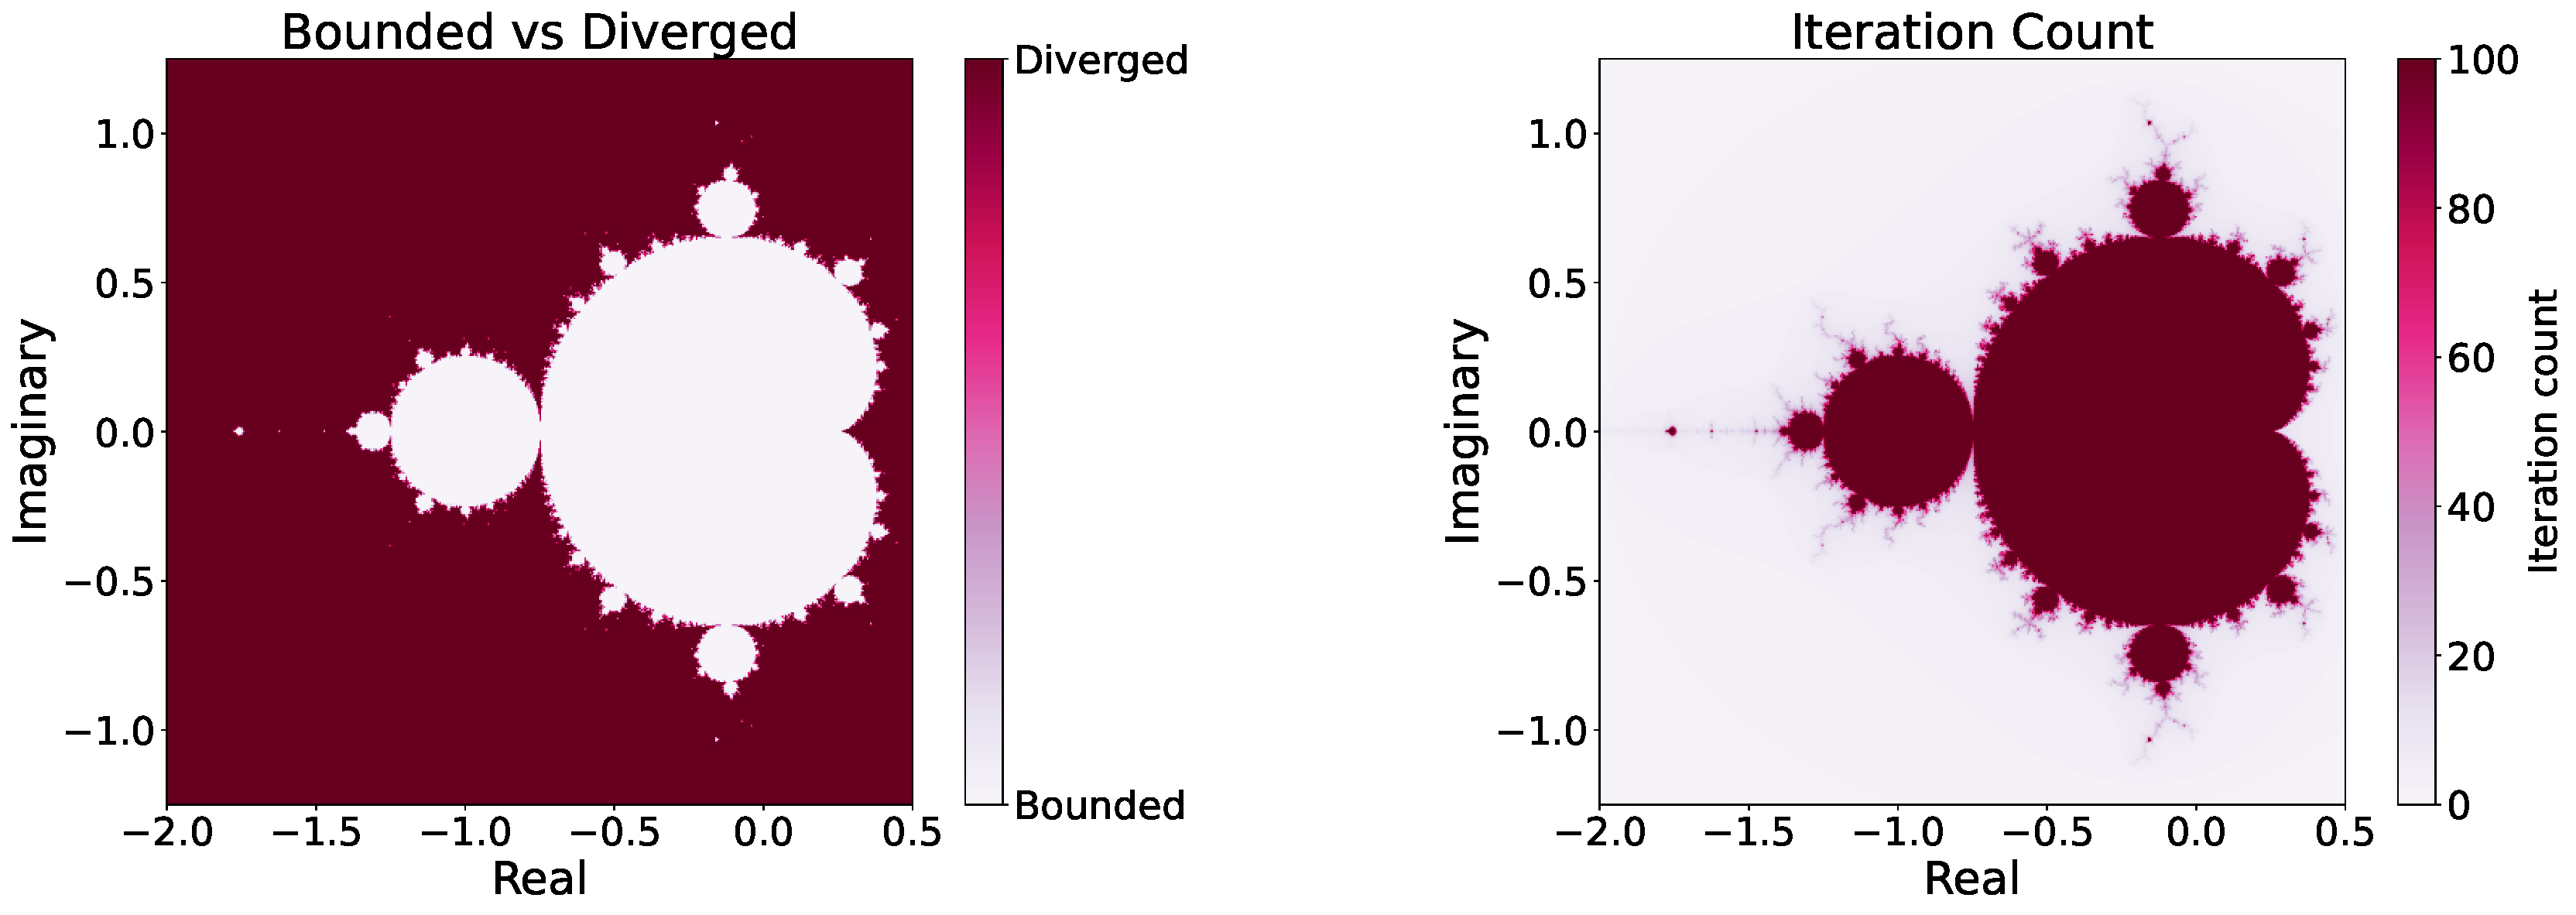
\includegraphics[width=0.9\textwidth]{Mandelbrot_Set.pdf}
    \caption{Two representations of the Mandelbrot set. The left image shows which points $c$ diverge and which remain bounded. The right image shows the iteration number at which each diverging point first satisfies $|z_n| > 2$.}
    \label{fig:mandelbrot}
\end{figure}

\section*{Question 2: The Lorenz System}

The Lorenz system is a set of three coupled nonlinear differential equations originally developed as a simplified model of atmospheric convection. The variables $X$, $Y$, and $Z$ represent the amplitudes of three retained Fourier modes in Lorenz's truncated model. Their time evolution is governed by
\begin{align}
    \dot{X} &= -\sigma(X - Y), \label{eq:lorenz_x}\\
    \dot{Y} &= rX - Y - XZ, \label{eq:lorenz_y}\\
    \dot{Z} &= -bZ + XY, \label{eq:lorenz_z}
\end{align}
where $\dot{X}$, $\dot{Y}$, and $\dot{Z}$ denote derivatives with respect to time. The parameters $\sigma$, $r$, and $b$ are dimensionless constants: $\sigma$ is the Prandtl number, $r$ is the Rayleigh number, and $b$ is a dimensionless length-scale parameter.

I first wrote a function, \texttt{lorenz}, in a separate file, \texttt{function\_q2.py}, and imported it into the notebook using \texttt{from function\_q2 import lorenz}. This function calculates the derivatives given by Equations~\ref{eq:lorenz_x}--\ref{eq:lorenz_z}. I then used \texttt{solve\_ivp} from \texttt{scipy.integrate} with parameter values $(\sigma, r, b) = (10, 28, 8/3)$ and initial conditions $W_0 = (0, 1, 0)$. The system was integrated to $t = 60$ with a maximum step size of $\Delta t = 0.01$.

These parameter values and initial conditions were chosen to reproduce the figures in Lorenz's original paper \citep{lorenz1963}.

Figure~\ref{fig:lorenz1} reproduces Lorenz's Figure~1, showing $Y$ as a function of iteration number $N = t/\Delta t$ for the first 3000 iterations. The system initially oscillates regularly before transitioning to chaotic behaviour.

\begin{figure}[H]
    \centering
    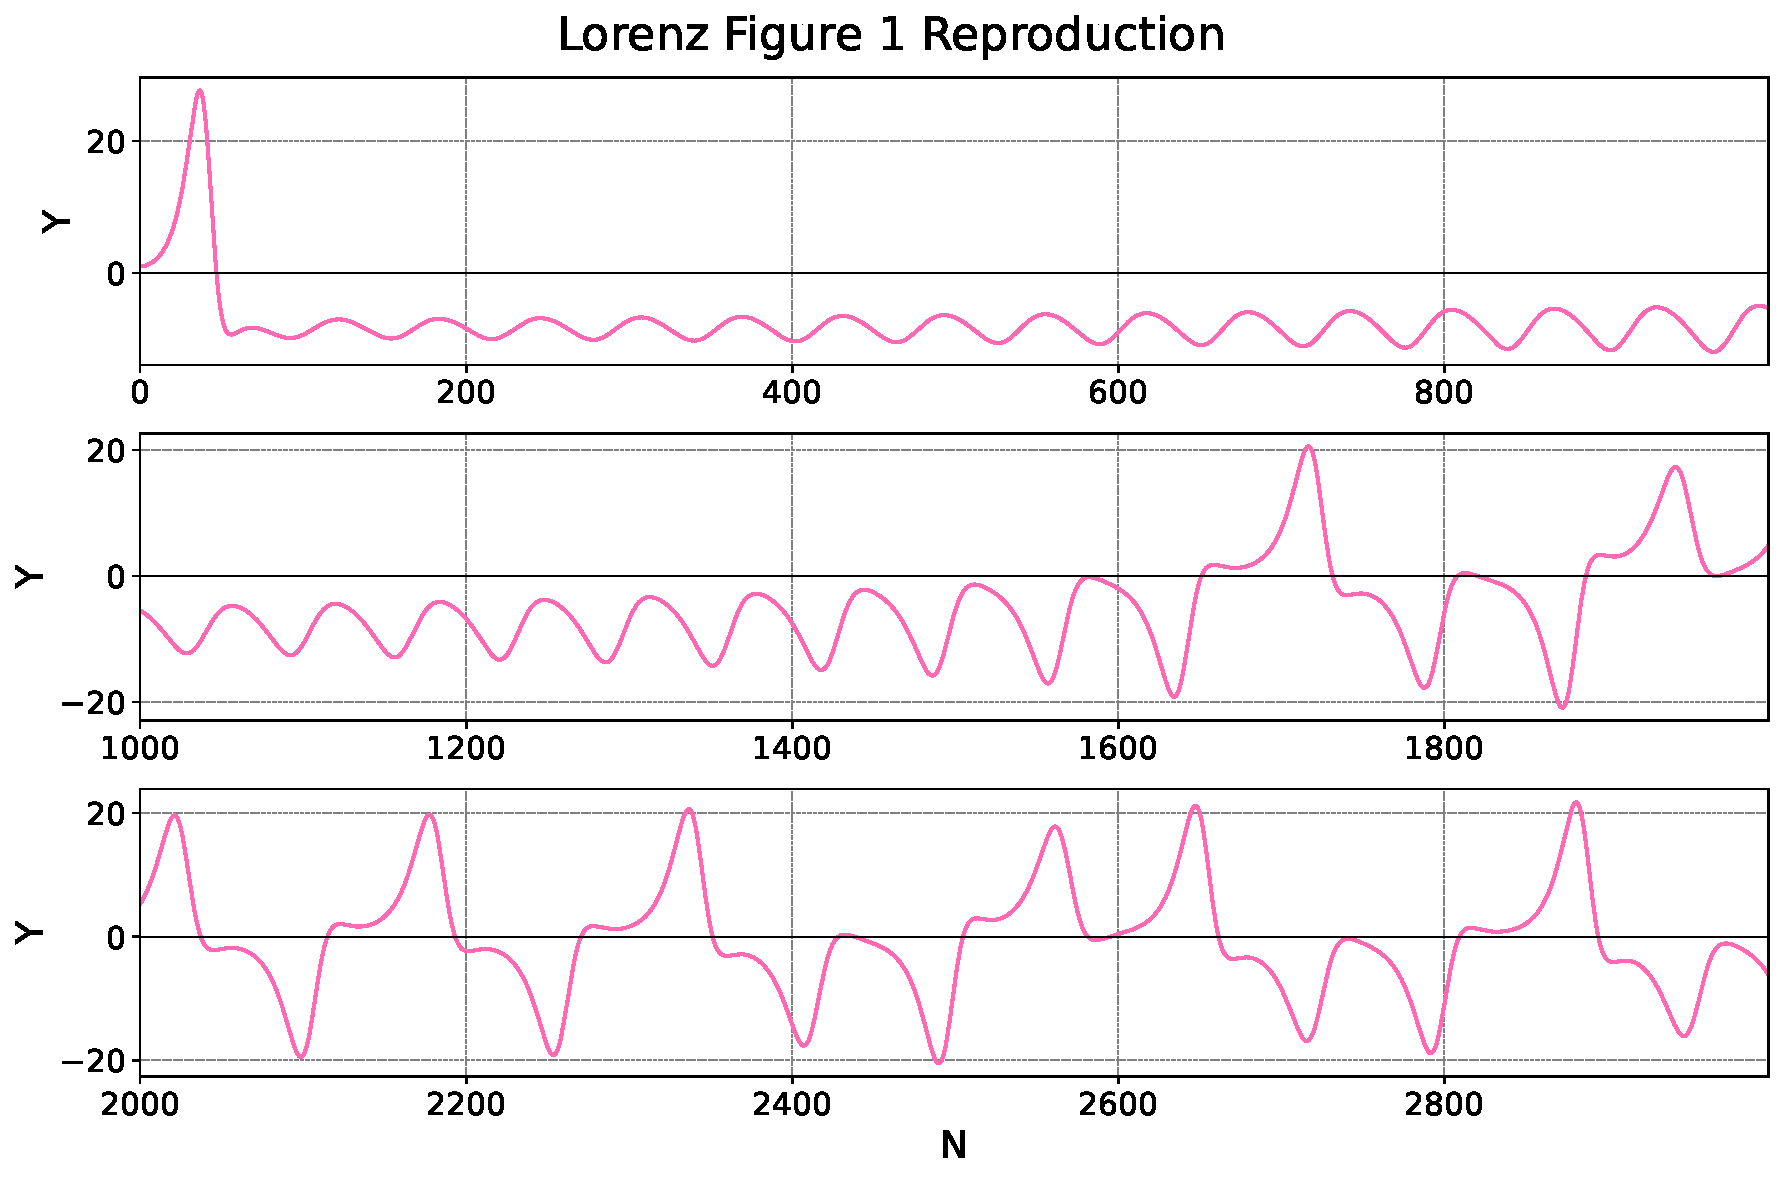
\includegraphics[width=0.8\textwidth]{Lorenz_1.pdf}
    \caption{Reproduction of Lorenz's Figure~1: $Y$ as a function of iteration number $N$ for the first 3000 iterations.}
    \label{fig:lorenz1}
\end{figure}

Figure~\ref{fig:lorenz2} reproduces Lorenz's Figure~2, showing the trajectory in phase space projected onto the $Y$-$Z$ and $X$-$Y$ planes for iterations 1400 to 1900. The spiral structure around the two steady convection states $C$ and $C'$ is clearly visible. An important note is that I inverted the x axis in order to match Lorenz's Figure~2.

\begin{figure}[H]
    \centering
    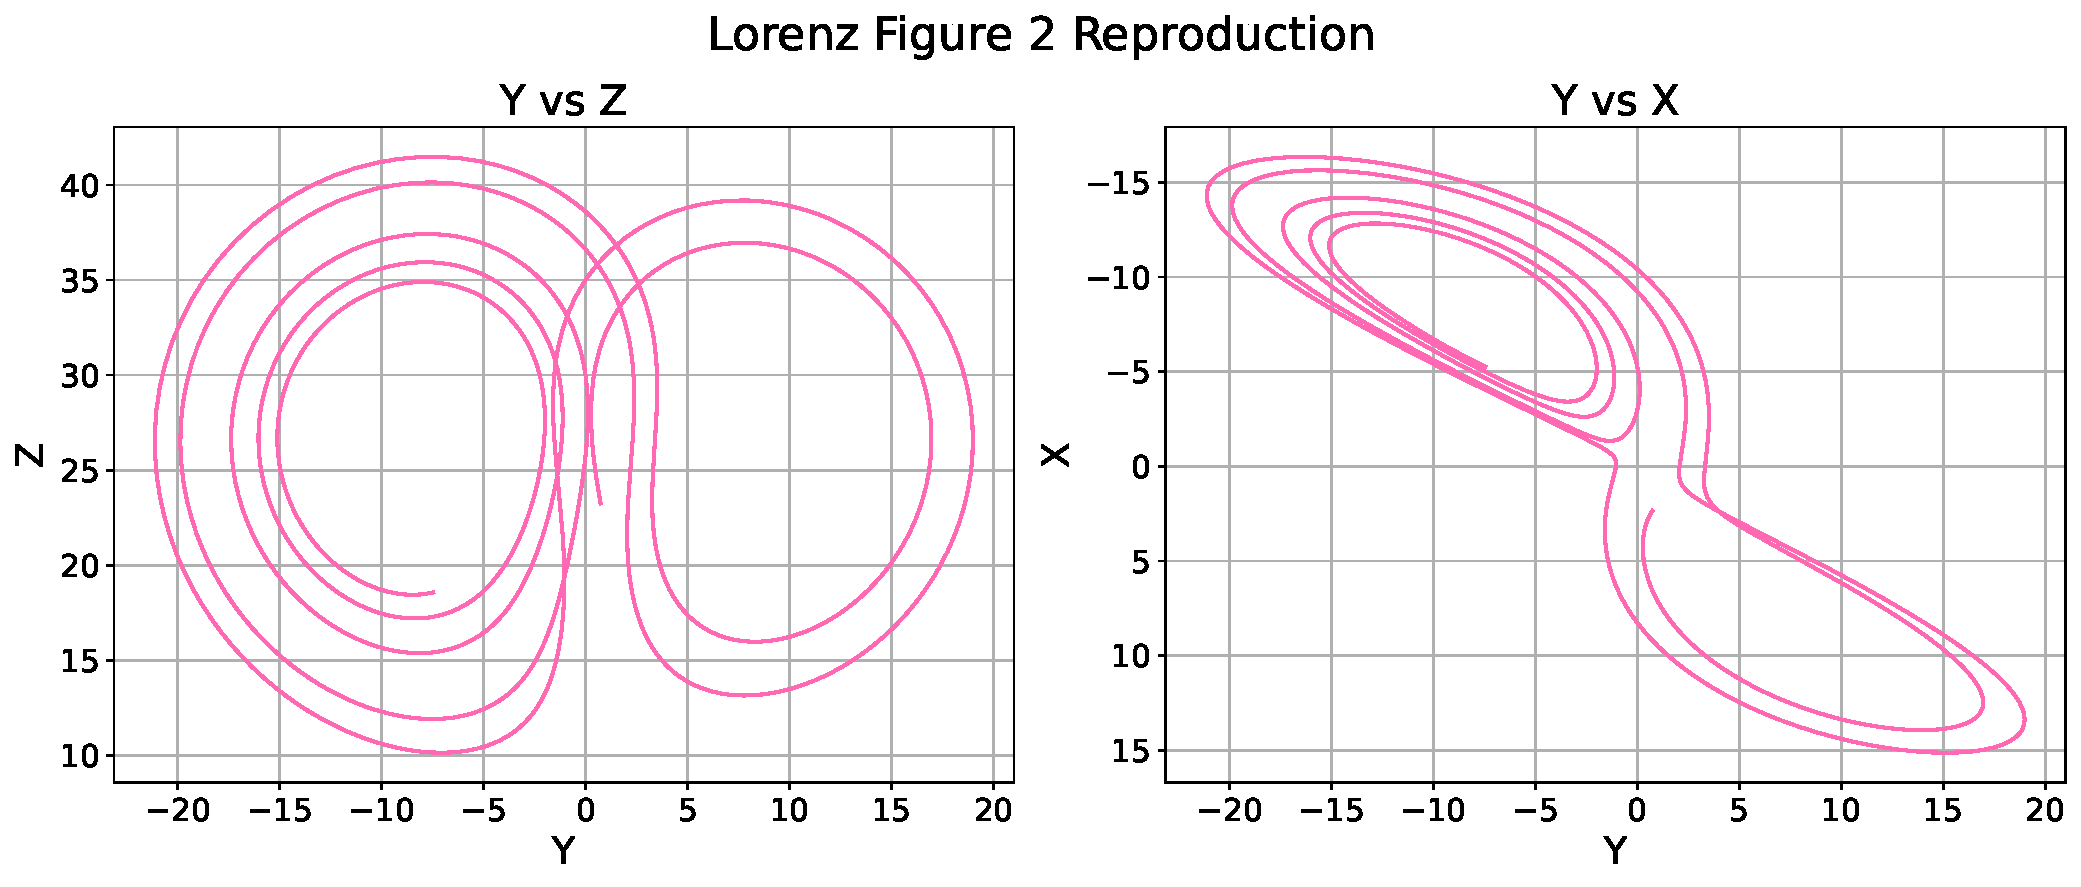
\includegraphics[width=0.9\textwidth]{Lorenz_2.pdf}
    \caption{Reproduction of Lorenz's Figure~2, showing phase-space projections from iteration 1400 to 1900. The left panel shows the $Y$-$Z$ projection and the right panel shows the $Y$-$X$ projection.}
    \label{fig:lorenz2}
\end{figure}

To test the sensitivity of the Lorenz system to initial conditions, I integrated two trajectories with initial conditions differing by only $10^{-8}$ in $Y$. This comparison quantifies how a very small uncertainty in the initial state propagates over time. Figure~\ref{fig:sensitivity} shows the distance between the two solutions as a function of time. The distance initially remains small, then grows rapidly before eventually saturating once the two trajectories become separated on the scale of the attractor. This behaviour demonstrates that the Lorenz system is chaotic and highly sensitive to initial conditions, meaning that long-term prediction becomes practically impossible even when the initial uncertainty is extremely small.

\begin{figure}[H]
    \centering
    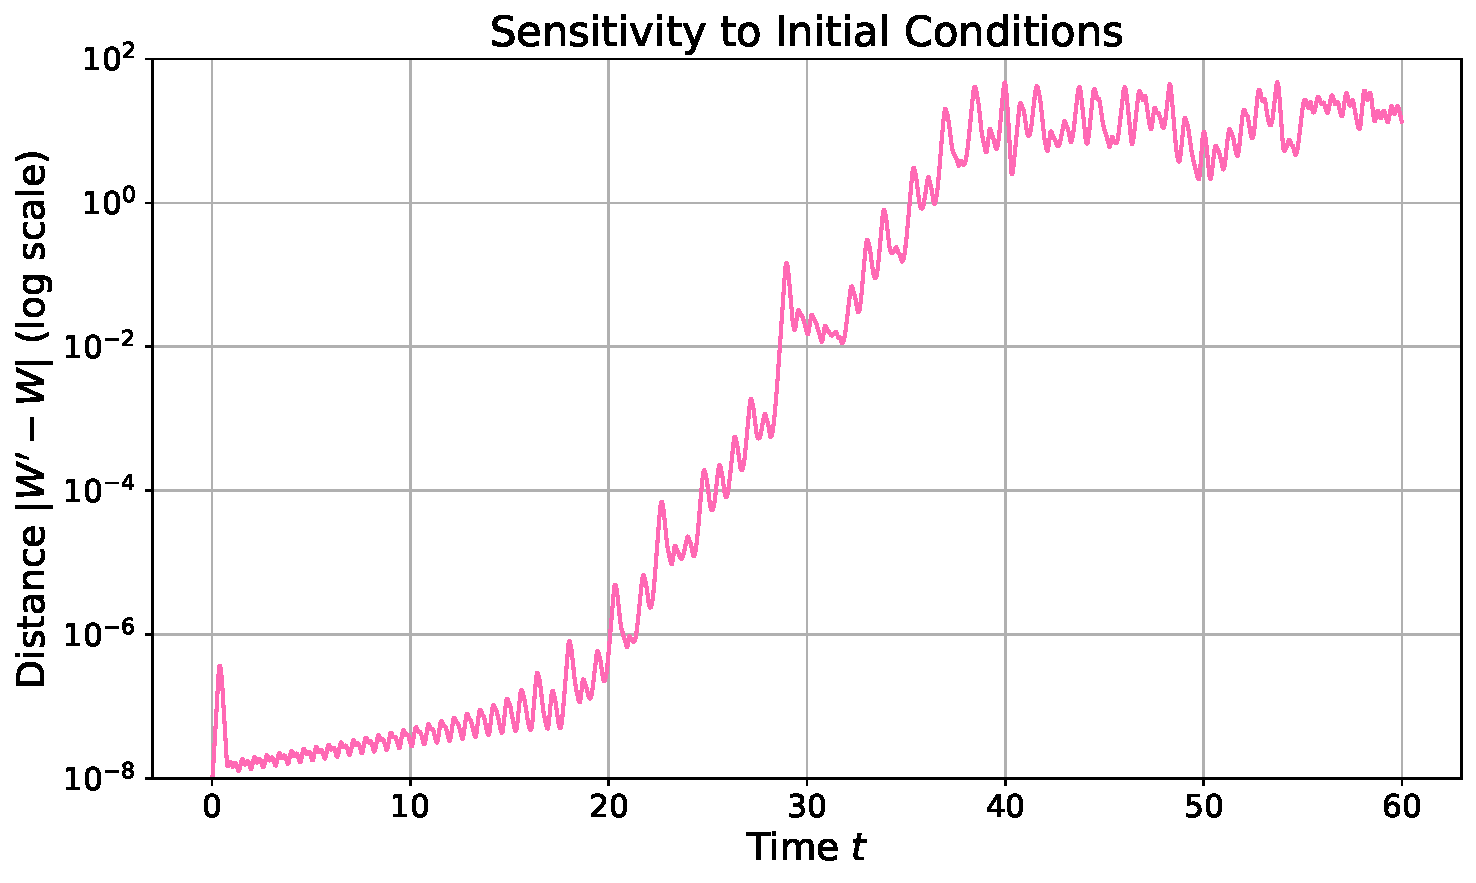
\includegraphics[width=0.8\textwidth]{Sensitivity.pdf}
    \caption{Distance between two Lorenz-system solutions with initial conditions differing by $10^{-8}$ in $Y$, shown as a function of time on a semilog scale.}
    \label{fig:sensitivity}
\end{figure}

\section*{Conclusion}

In this assignment, I investigated two examples of nonlinear systems that exhibit complex behaviour. For the Mandelbrot set, iterating the map $z_{n+1} = z_n^2 + c$ showed how a simple recurrence relation can produce a highly detailed fractal boundary between bounded and diverging points. For the Lorenz system, numerical integration reproduced Lorenz's original figures and demonstrated the system's sensitivity to initial conditions. The rapid growth of small initial differences illustrates the central idea of chaos: deterministic equations can still become unpredictable over long times. In the context of Lorenz's original atmospheric model, this explains why weather prediction becomes increasingly unreliable as small errors in the initial state grow with time.

\begin{thebibliography}{9}

\bibitem{lorenz1963}
Lorenz, E. N. (1963). Deterministic nonperiodic flow.
\textit{Journal of the Atmospheric Sciences}, 20(2), 130--141.

\bibitem{mandelbrot1980}
Mandelbrot, B. B. (1980). Fractal aspects of the iteration of 
$z \to \lambda z(1-z)$ for complex $\lambda$ and $z$. 
\textit{Annals of the New York Academy of Sciences}, 357, 249--259.

\end{thebibliography}

\end{document}